\documentclass[aspectratio=169]{beamer}
\usetheme{Madrid}
\usecolortheme{whale}
\setbeamertemplate{navigation symbols}{}
\setbeamertemplate{caption}[numbered]
\setbeamerfont{title}{size=\Large}
\setbeamerfont{subtitle}{size=\small}
\setbeamerfont{frametitle}{size=\large}
\setbeamerfont{block title}{size=\small}
\setbeamertemplate{blocks}[rounded][shadow=true]
\setbeamersize{text margin left=0.7cm,text margin right=0.7cm}

\title{Human-Centric Design for Data-Driven Decision Support}
\subtitle{A 20-slide presentation of the SFU Master\textquotesingle s thesis}
\author{Mehdi Vahabisani}
\institute{School of Interactive Arts and Technology\textbackslash\\ Simon Fraser University}
\date{\today}

\begin{document}

\begin{frame}[plain]
  \titlepage
\end{frame}

\begin{frame}{Thesis at a Glance}
  \begin{columns}[T,onlytextwidth]
    \column{0.48\textwidth}
    \begin{block}{Core argument}
      \begin{itemize}
        \item Decision support must be task-aware.
        \item No single technique is sufficient.
        \item Human agency remains essential.
        \item Causal, predictive, and optimization tools complement each other.
      \end{itemize}
    \end{block}
    \column{0.52\textwidth}
    \begin{block}{Research contribution}
      \begin{itemize}
        \item Integrates data-driven tools across the decision process.
        \item Links techniques to decision stages, users, and tasks.
        \item Supports reasoning rather than replacing human judgment.
        \item Provides a framework for organizational decision support.
      \end{itemize}
    \end{block}
  \end{columns}
\end{frame}

\begin{frame}{The Research Problem}
  \begin{columns}[T,onlytextwidth]
    \column{0.48\textwidth}
    \begin{block}{Key challenges}
      \begin{itemize}
        \item Data-driven tools are often applied separately.
        \item Correlations may be mistaken for causal effects.
        \item Large analytical outputs can create cognitive overload.
        \item Black-box models may reduce trust and confidence.
      \end{itemize}
    \end{block}
    \column{0.52\textwidth}
    \centering
    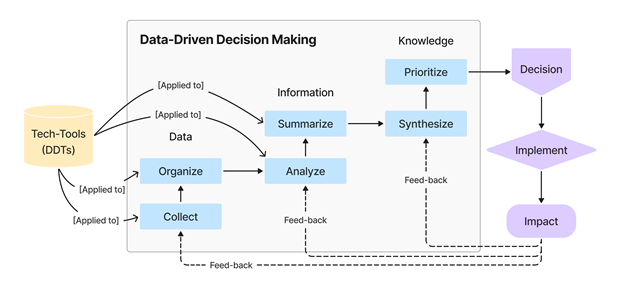
\includegraphics[width=0.95\textwidth]{Figures/DDDMProcess.png}
    \captionof{figure}{Conceptual data-driven decision-making process}
  \end{columns}
\end{frame}

\begin{frame}{Research Questions}
  \begin{block}{The thesis investigates four questions}
    \begin{enumerate}
      \item Which data-driven techniques support organizational decisions?
      \item How do these techniques augment decision-making?
      \item What role does causal reasoning play?
      \item How should tools be integrated for the user and task?
    \end{enumerate}
  \end{block}
  \centering
  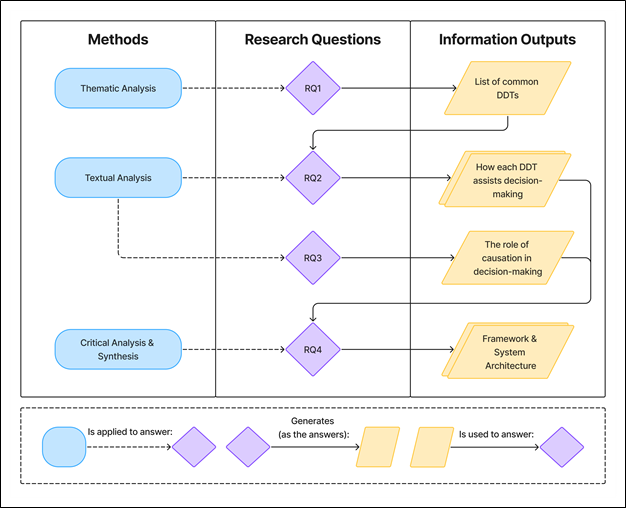
\includegraphics[width=0.8\textwidth]{Figures/ResearchProcess.png}
\end{frame}

\begin{frame}{Research Methodology}
  \begin{columns}[T,onlytextwidth]
    \column{0.48\textwidth}
    \begin{block}{Approach}
      \begin{itemize}
        \item Review data-driven decision-making literature.
        \item Classify recurring techniques.
        \item Analyze causal reasoning and human factors.
        \item Synthesize a human-and-task-centered framework.
      \end{itemize}
    \end{block}
    \column{0.52\textwidth}
    \centering
    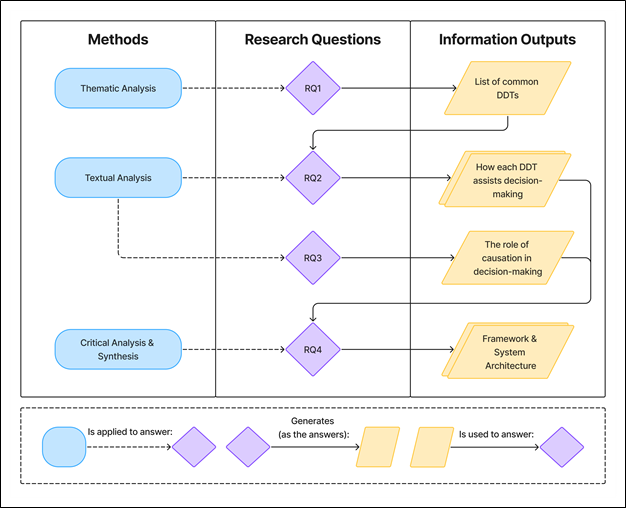
\includegraphics[width=0.95\textwidth]{Figures/ResearchProcess.png}
  \end{columns}
\end{frame}

\begin{frame}{The Literature Landscape}
  \begin{columns}[T,onlytextwidth]
    \column{0.35\textwidth}
    \begin{itemize}
      \item Machine learning
      \item Traditional statistics
      \item Data visualization
      \item Natural language models
      \item Mathematical optimization
      \item Simulation
    \end{itemize}
    \column{0.65\textwidth}
    \centering
    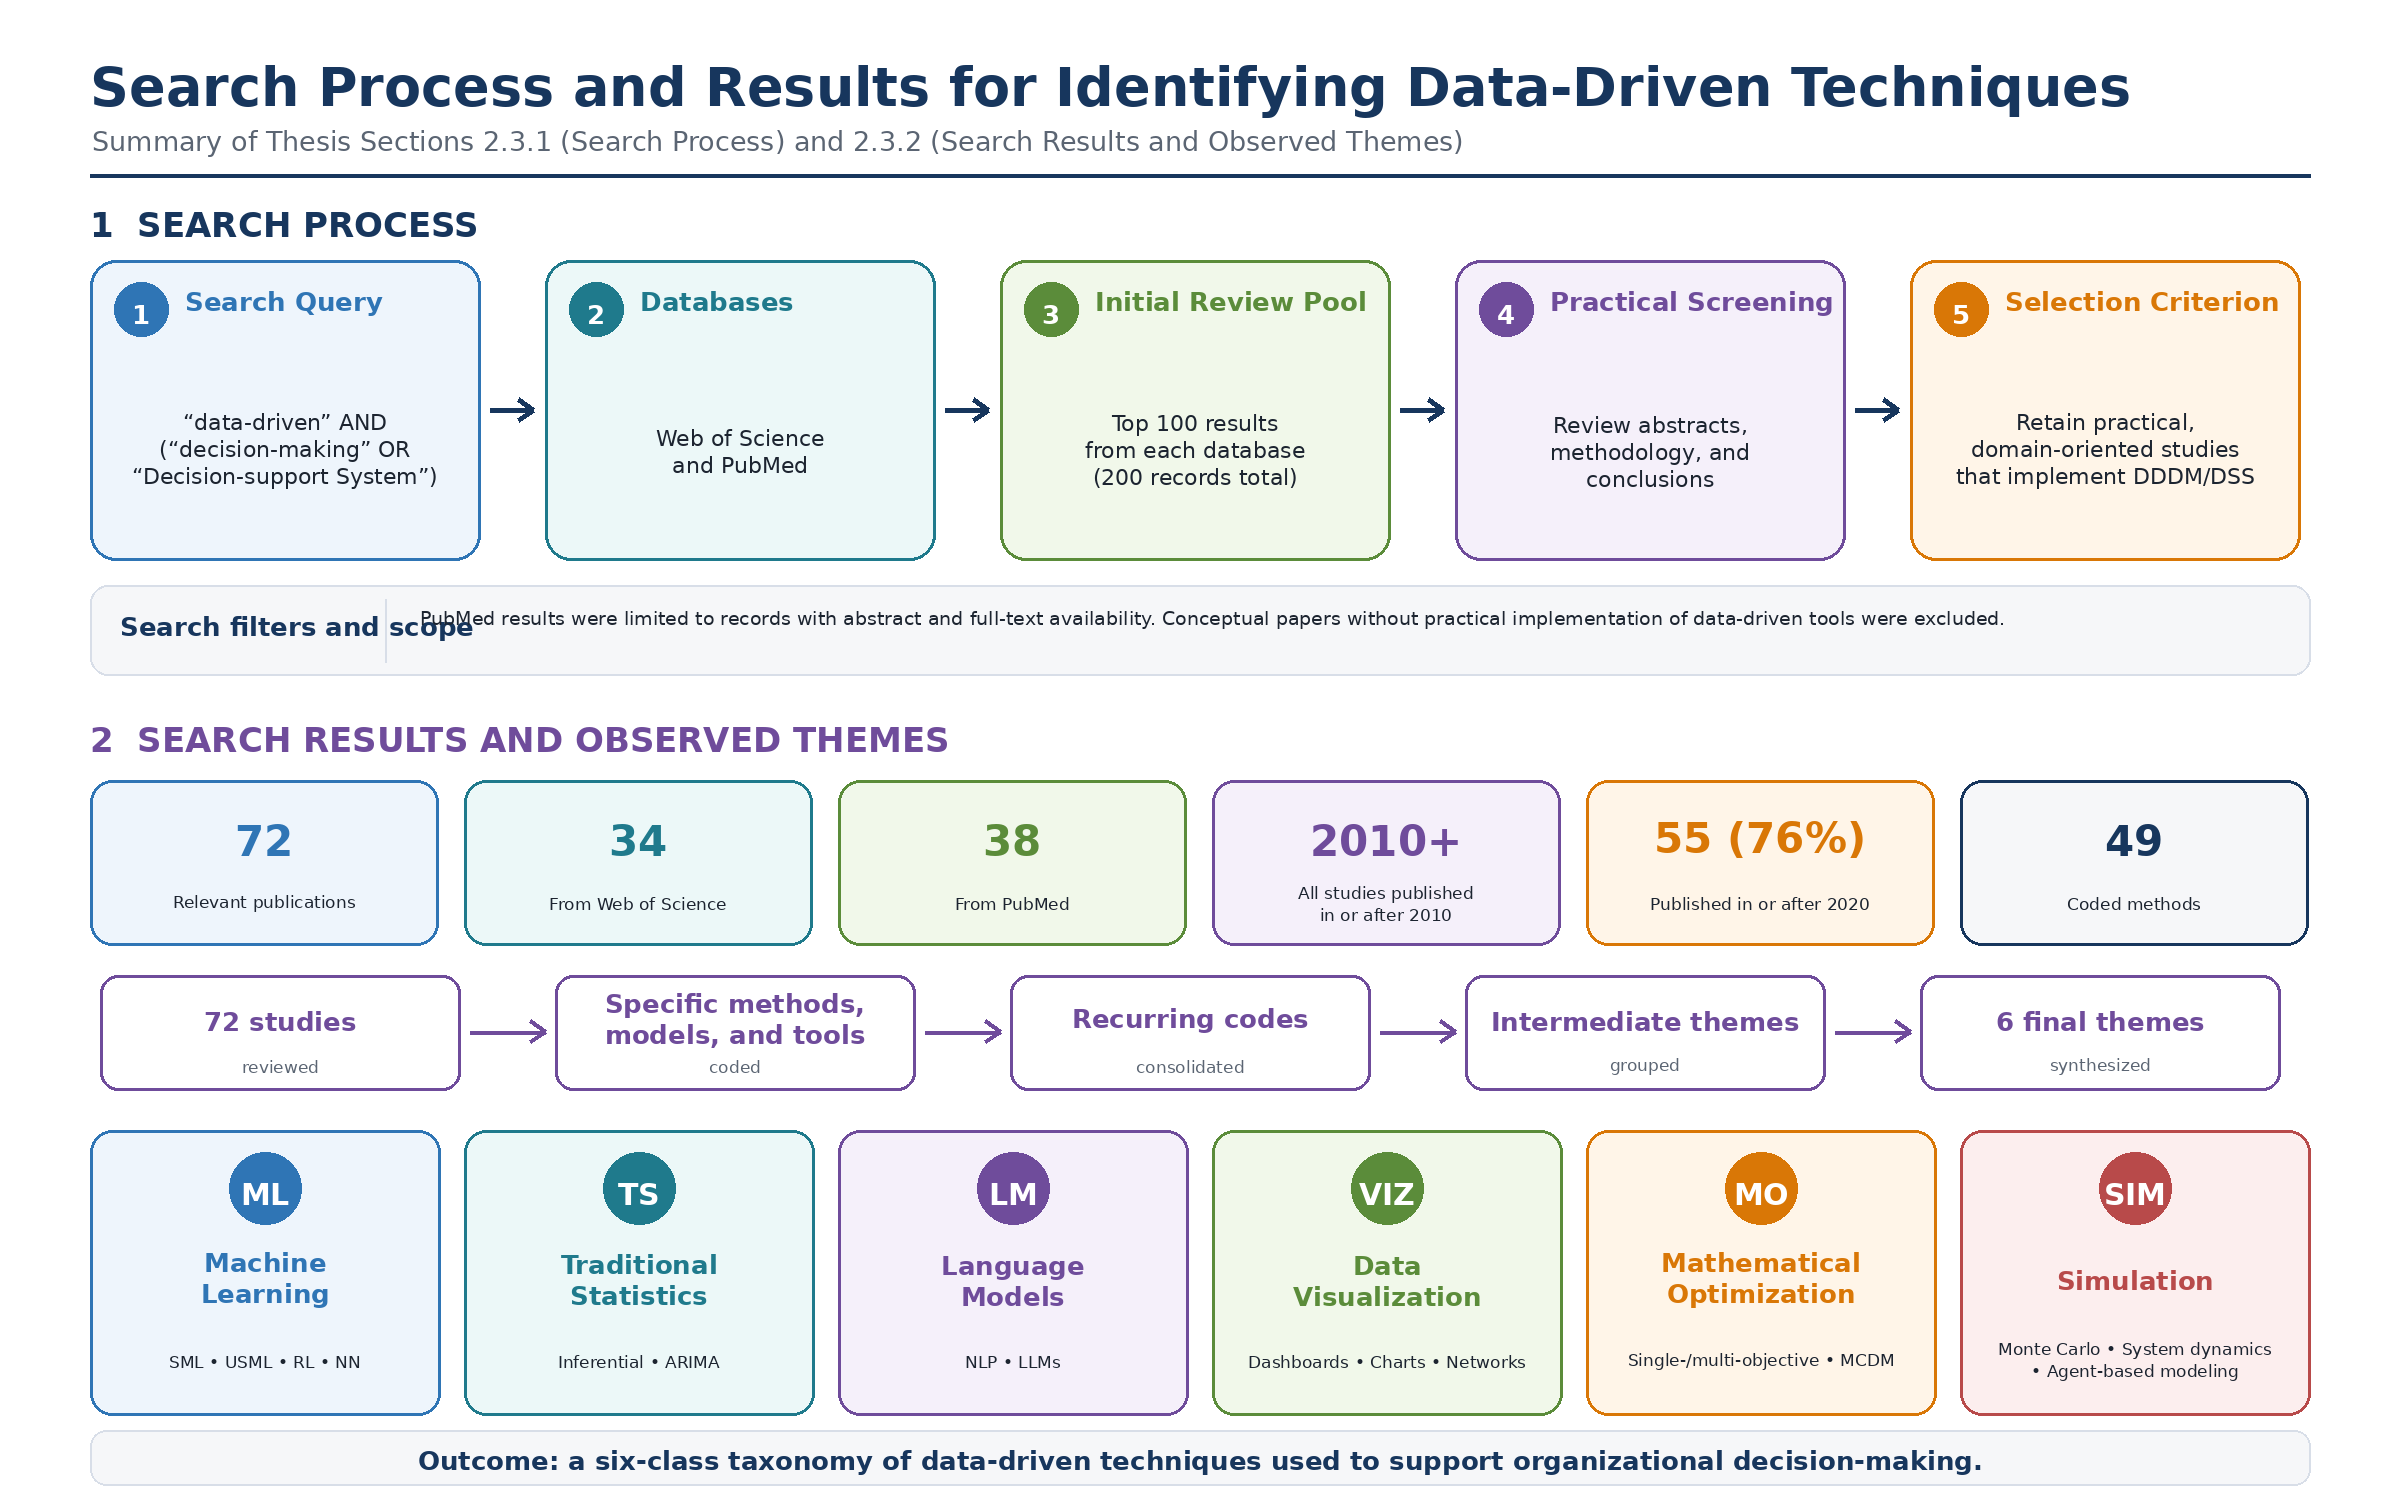
\includegraphics[width=0.98\textwidth]{Figures/DDDMLitReview_search_summary.png}
  \end{columns}
\end{frame}

\begin{frame}{The Decision-Making Process}
  \begin{columns}[T,onlytextwidth]
    \column{0.38\textwidth}
    \begin{block}{Three stages}
      \textbf{Intelligence}: detect and frame the problem.\newline
      \textbf{Design}: define criteria, variables, and alternatives.\newline
      \textbf{Choice}: evaluate, compare, and select.
    \end{block}
    \column{0.62\textwidth}
    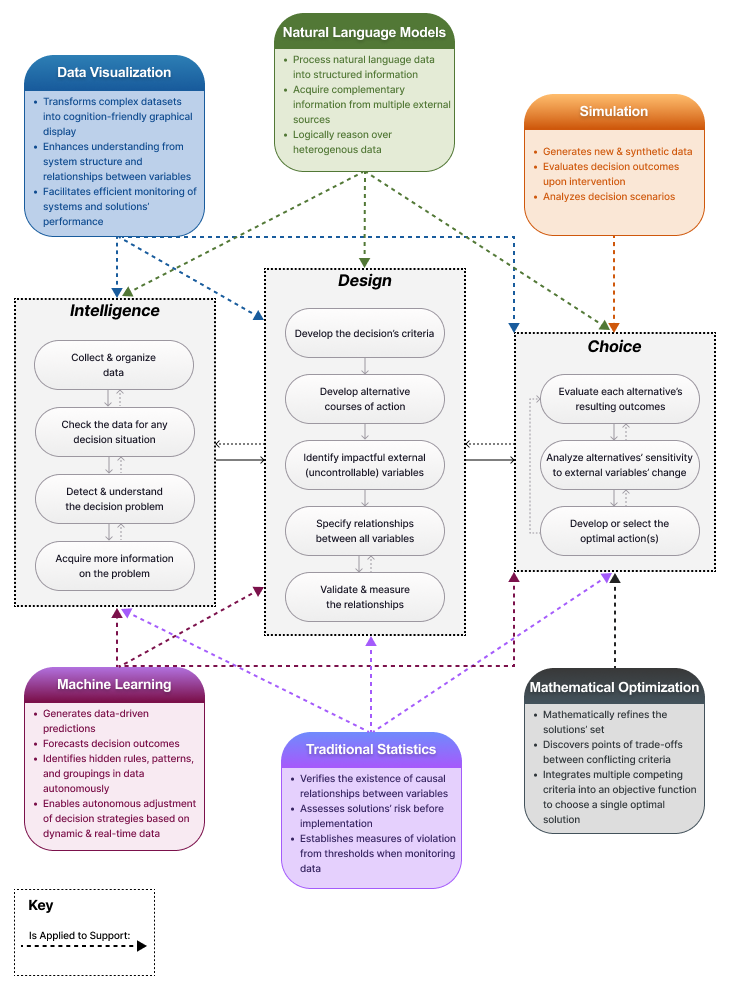
\includegraphics[width=0.95\textwidth]{Figures/DDTAssignment.png}
  \end{columns}
\end{frame}

\begin{frame}{Machine Learning}
  \begin{columns}[T,onlytextwidth]
    \column{0.45\textwidth}
    \begin{itemize}
      \item Supervised learning: prediction and classification.
      \item Unsupervised learning: clustering and anomaly detection.
      \item Reinforcement learning: adaptive policies.
      \item Explainable models: transparent recommendations.
    \end{itemize}
    \column{0.55\textwidth}
    \centering
    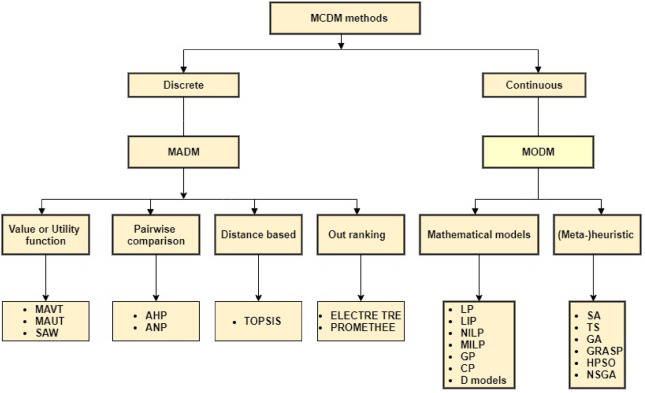
\includegraphics[width=0.9\textwidth]{Figures/MCDMTree.jpg}
  \end{columns}
\end{frame}

\begin{frame}{Traditional Statistics}
  \begin{columns}[T,onlytextwidth]
    \column{0.45\textwidth}
    \begin{itemize}
      \item Descriptive and exploratory analysis.
      \item Hypothesis testing and statistical significance.
      \item Forecasting and time-series analysis.
      \item Risk estimation and threshold monitoring.
    \end{itemize}
    \column{0.55\textwidth}
    \centering
    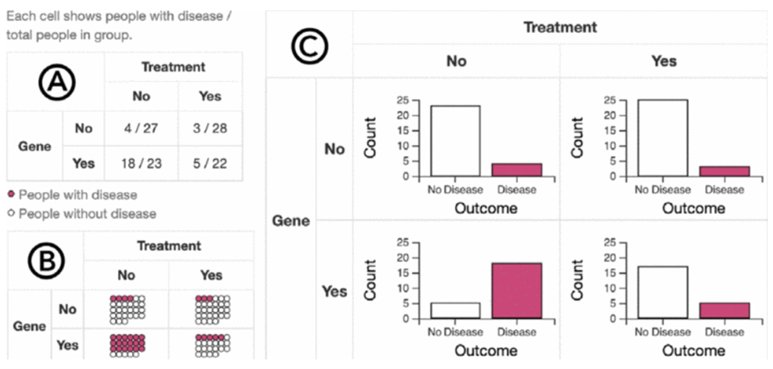
\includegraphics[width=0.9\textwidth]{Figures/ContingencyTables.png}
  \end{columns}
\end{frame}

\begin{frame}{Data Visualization}
  \begin{columns}[T,onlytextwidth]
    \column{0.45\textwidth}
    \begin{itemize}
      \item Pattern recognition.
      \item Alternative comparison.
      \item Temporal and spatial exploration.
      \item Interactive cross-filtering.
    \end{itemize}
    \column{0.55\textwidth}
    \centering
    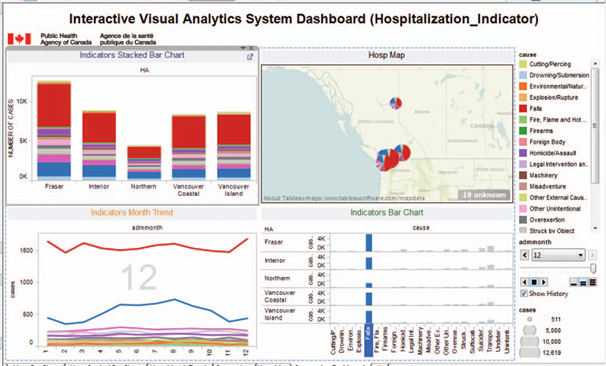
\includegraphics[width=0.9\textwidth]{Figures/VADashboardPublicHealth.png}
  \end{columns}
\end{frame}

\begin{frame}{Optimization and Simulation}
  \begin{columns}[T,onlytextwidth]
    \column{0.45\textwidth}
    \begin{itemize}
      \item Multi-objective optimization and Pareto trade-offs.
      \item MCDM for comparing alternatives across criteria.
      \item Simulation and scenario analysis.
      \item Stochastic models for uncertainty.
    \end{itemize}
    \column{0.55\textwidth}
    \centering
    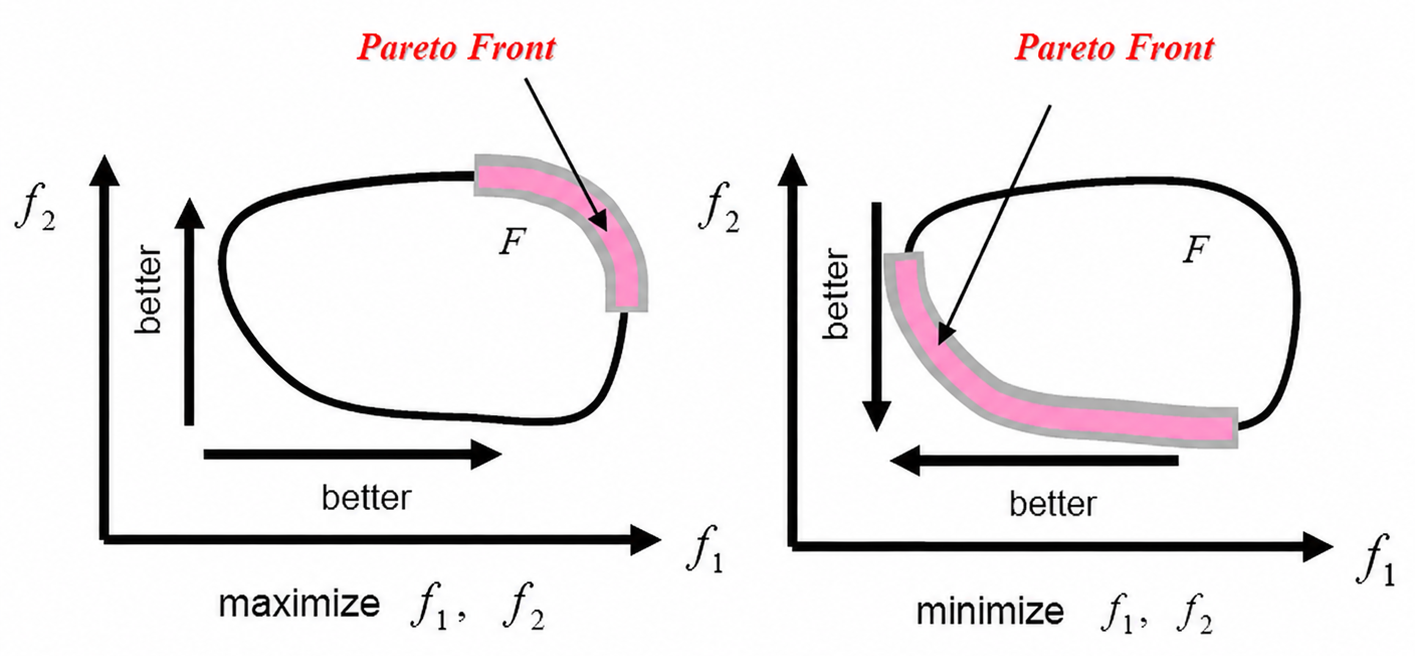
\includegraphics[width=0.9\textwidth]{Figures/Biobjective_VIZ.png}
  \end{columns}
\end{frame}

\begin{frame}{Causal Reasoning}
  \begin{columns}[T,onlytextwidth]
    \column{0.45\textwidth}
    \begin{itemize}
      \item Explains why outcomes occur.
      \item Distinguishes causes, effects, mediators, and confounders.
      \item Supports intervention planning.
      \item Enables action-oriented reasoning.
    \end{itemize}
    \column{0.55\textwidth}
    \centering
    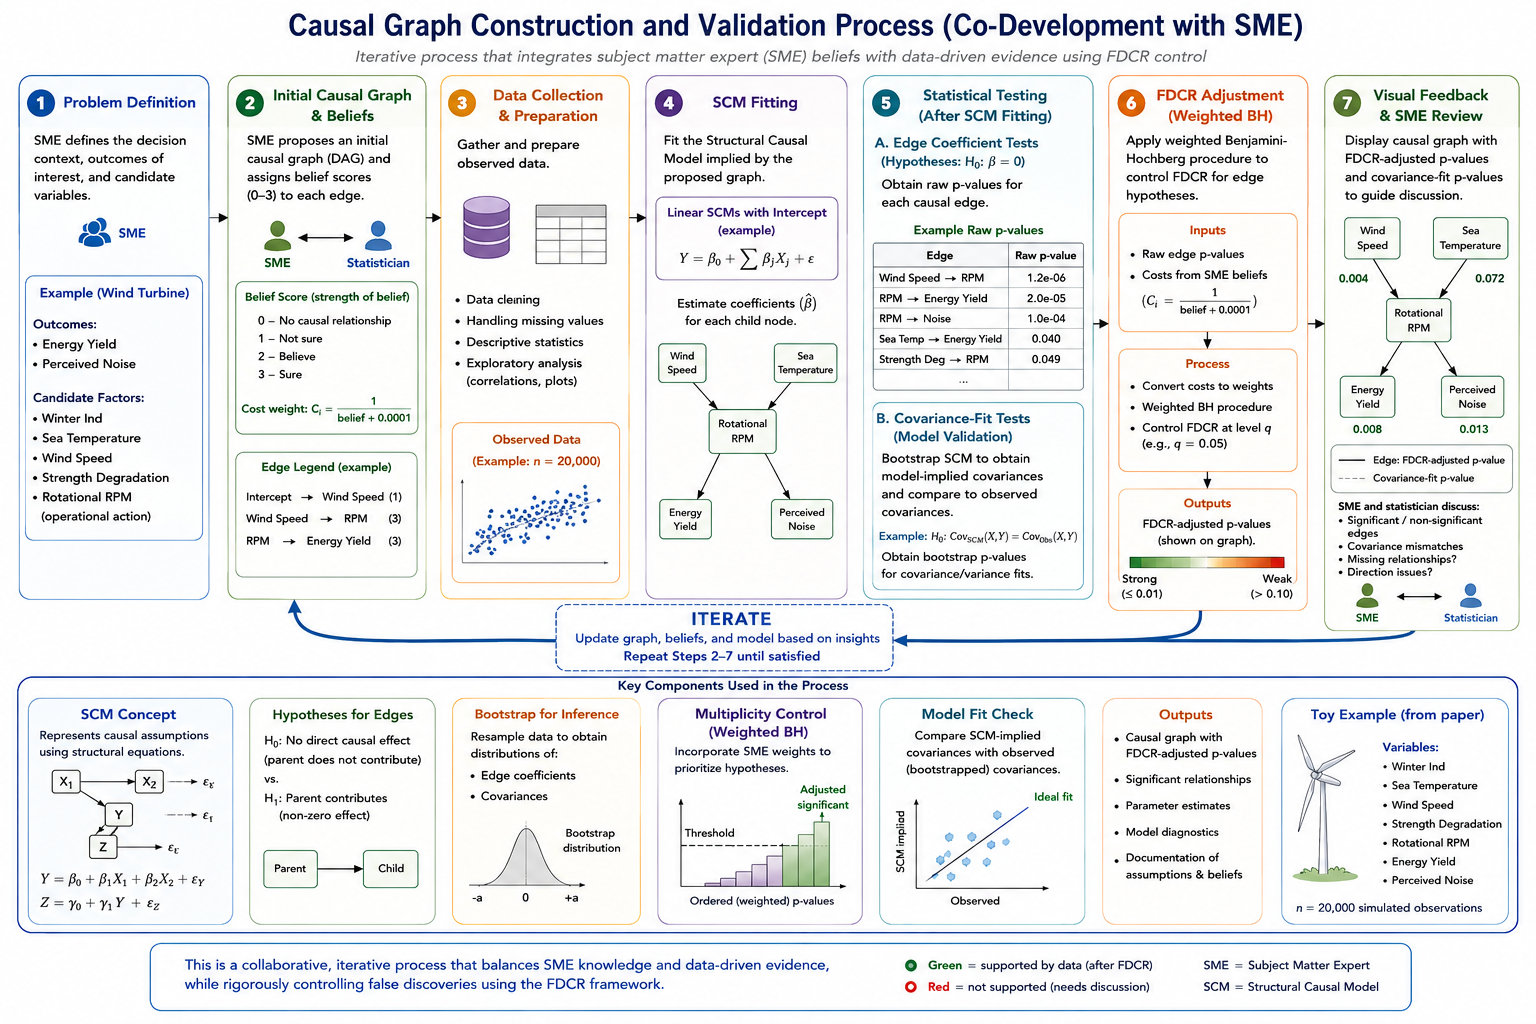
\includegraphics[width=0.95\textwidth]{Figures/CausalGraphConstructionProcess.png}
  \end{columns}
\end{frame}

\begin{frame}{Counterfactual Thinking}
  \begin{columns}[T,onlytextwidth]
    \column{0.45\textwidth}
    \begin{itemize}
      \item What would have happened without this action?
      \item Which action would have produced a better outcome?
      \item How robust is the selected option?
      \item How does uncertainty affect the comparison?
    \end{itemize}
    \column{0.55\textwidth}
    \centering
    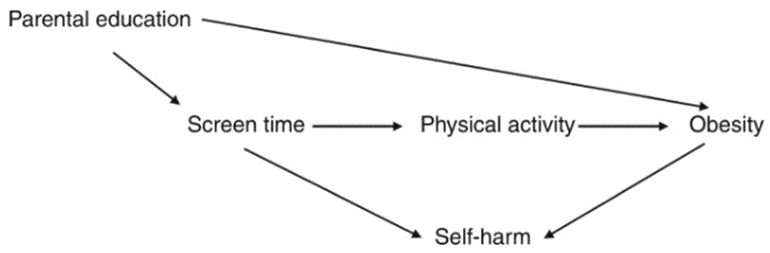
\includegraphics[width=0.95\textwidth]{Figures/DAGExample.png}
  \end{columns}
\end{frame}

\begin{frame}{Humanistic Factors}
  \begin{columns}[T,onlytextwidth]
    \column{0.45\textwidth}
    \begin{itemize}
      \item Working memory and attention.
      \item Domain knowledge and mental models.
      \item Expertise and experience.
      \item Decision style and cognitive preferences.
    \end{itemize}
    \column{0.55\textwidth}
    \begin{block}{Design implications}
      \begin{itemize}
        \item Analytical users benefit from structured evidence.
        \item Intuitive users may prefer fast guidance.
        \item Adaptive experts revise assumptions.
        \item Support should not enforce one decision style.
      \end{itemize}
    \end{block}
  \end{columns}
\end{frame}

\begin{frame}{Human-and-Task-Centered Framework}
  \centering
  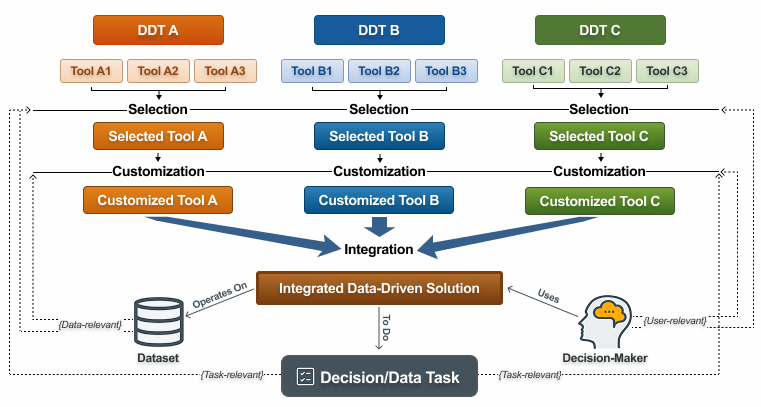
\includegraphics[width=0.96\textwidth]{Figures/ThreeLayerIntegration.png}
\end{frame}

\begin{frame}{Intelligence Stage}
  \centering
  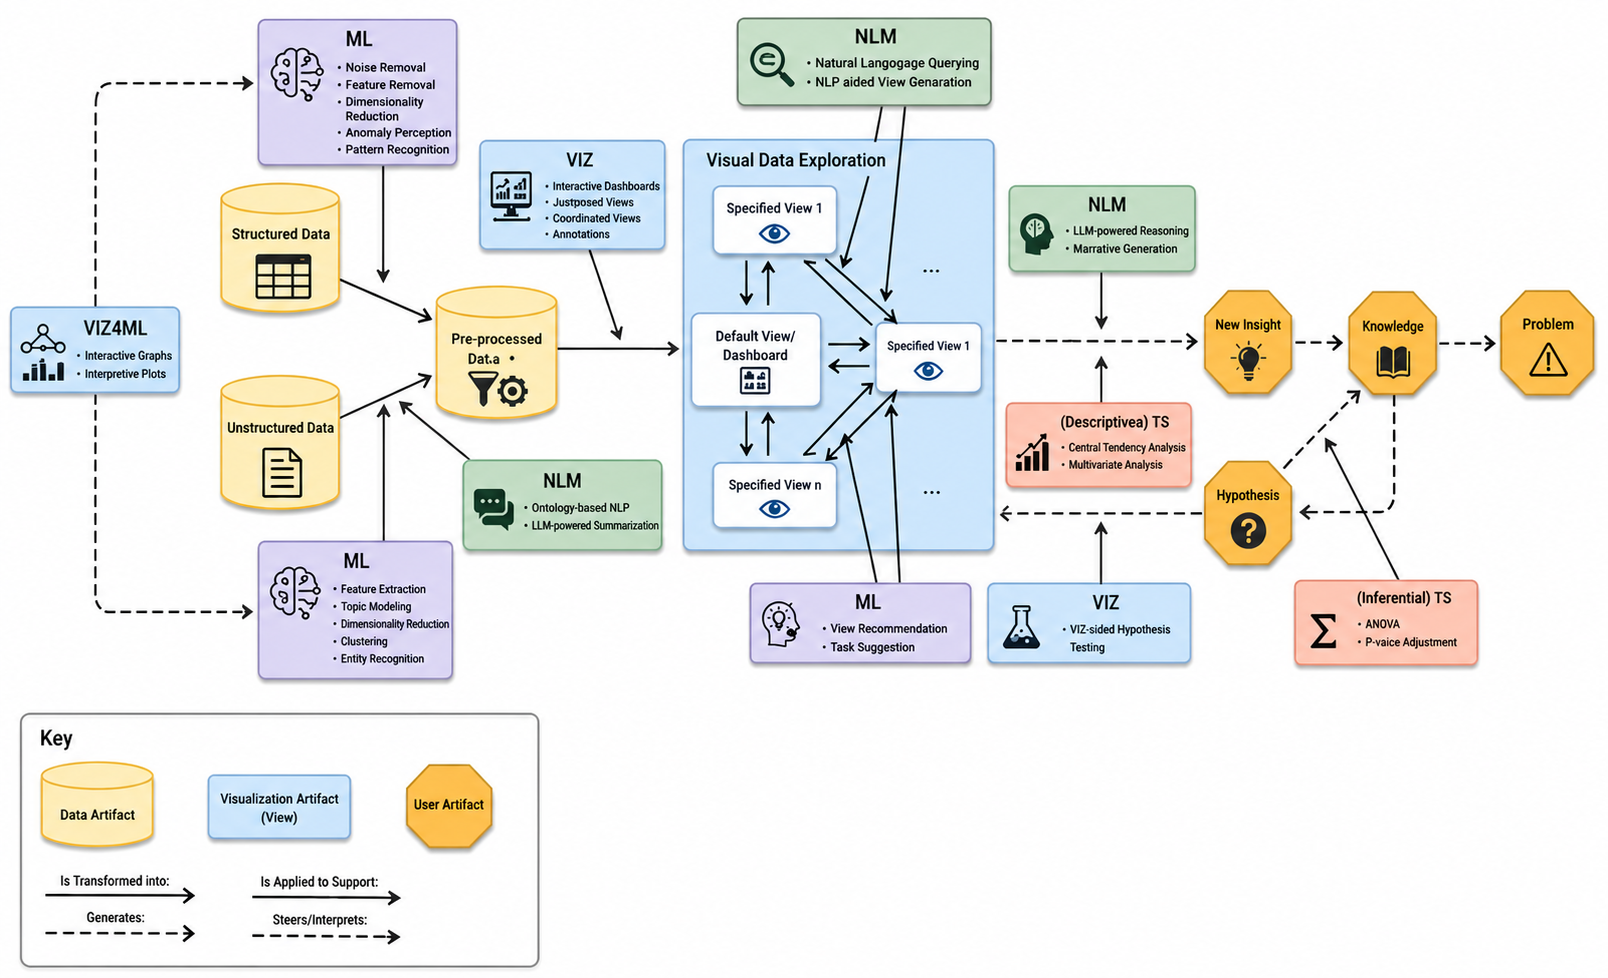
\includegraphics[width=0.98\textwidth]{Figures/IntelligenceWorkflow.png}
\end{frame}

\begin{frame}{Design Stage}
  \centering
  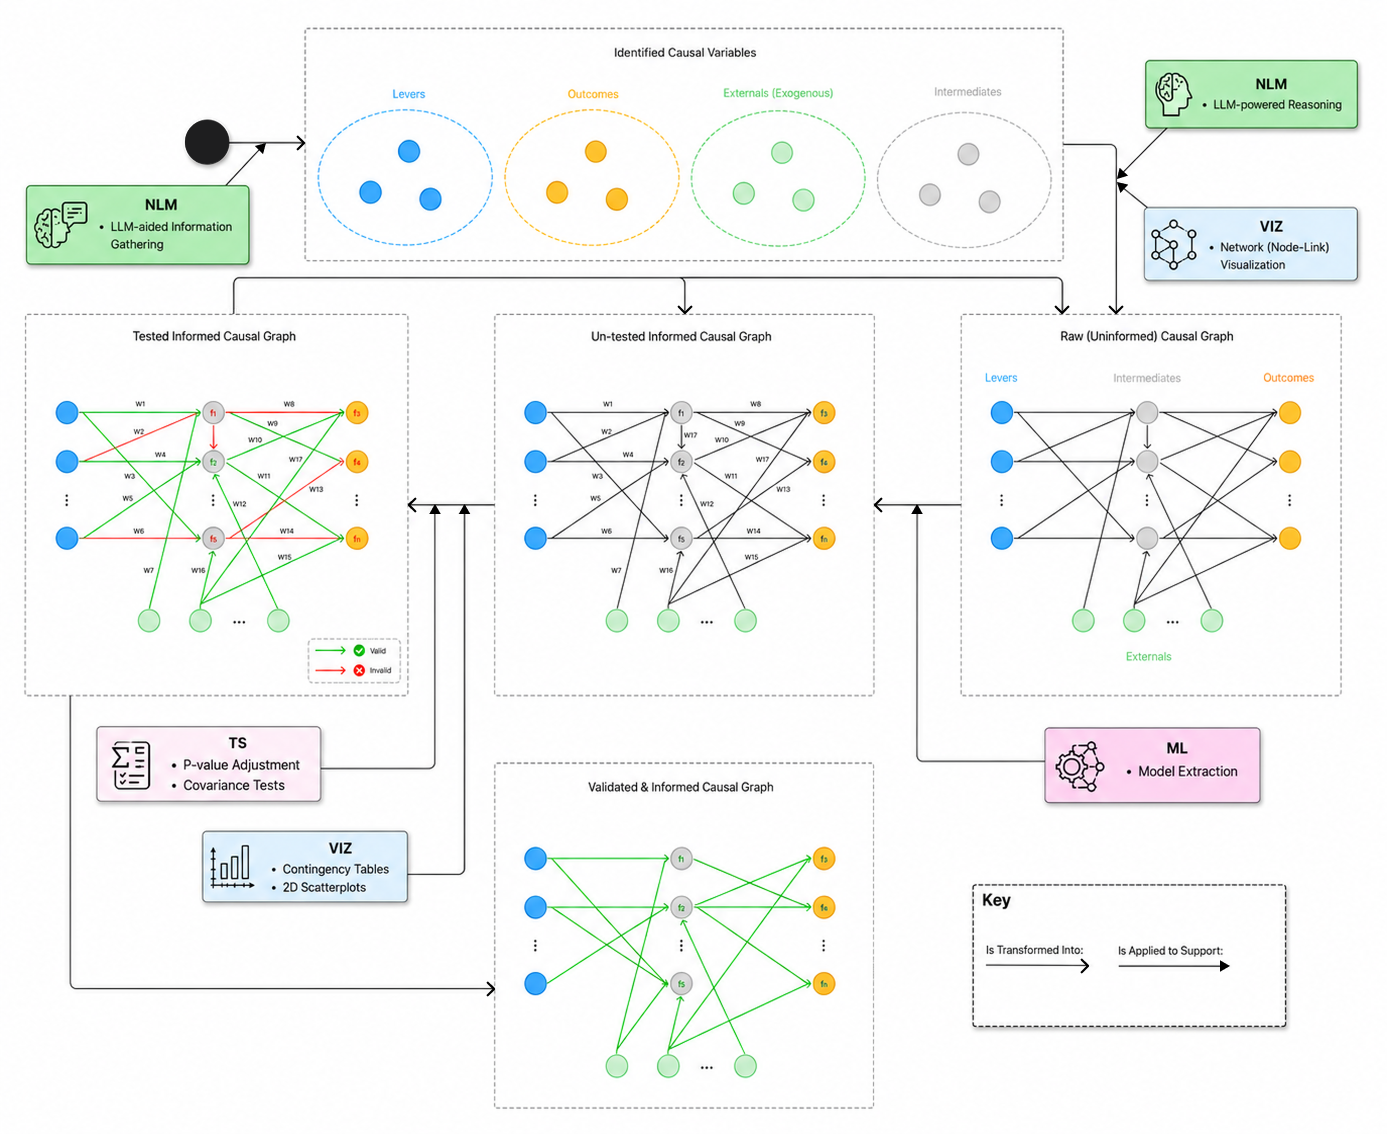
\includegraphics[width=0.98\textwidth]{Figures/DesignWorkflow_ArrowsAmplified.png}
\end{frame}

\begin{frame}{Choice Stage}
  \centering
  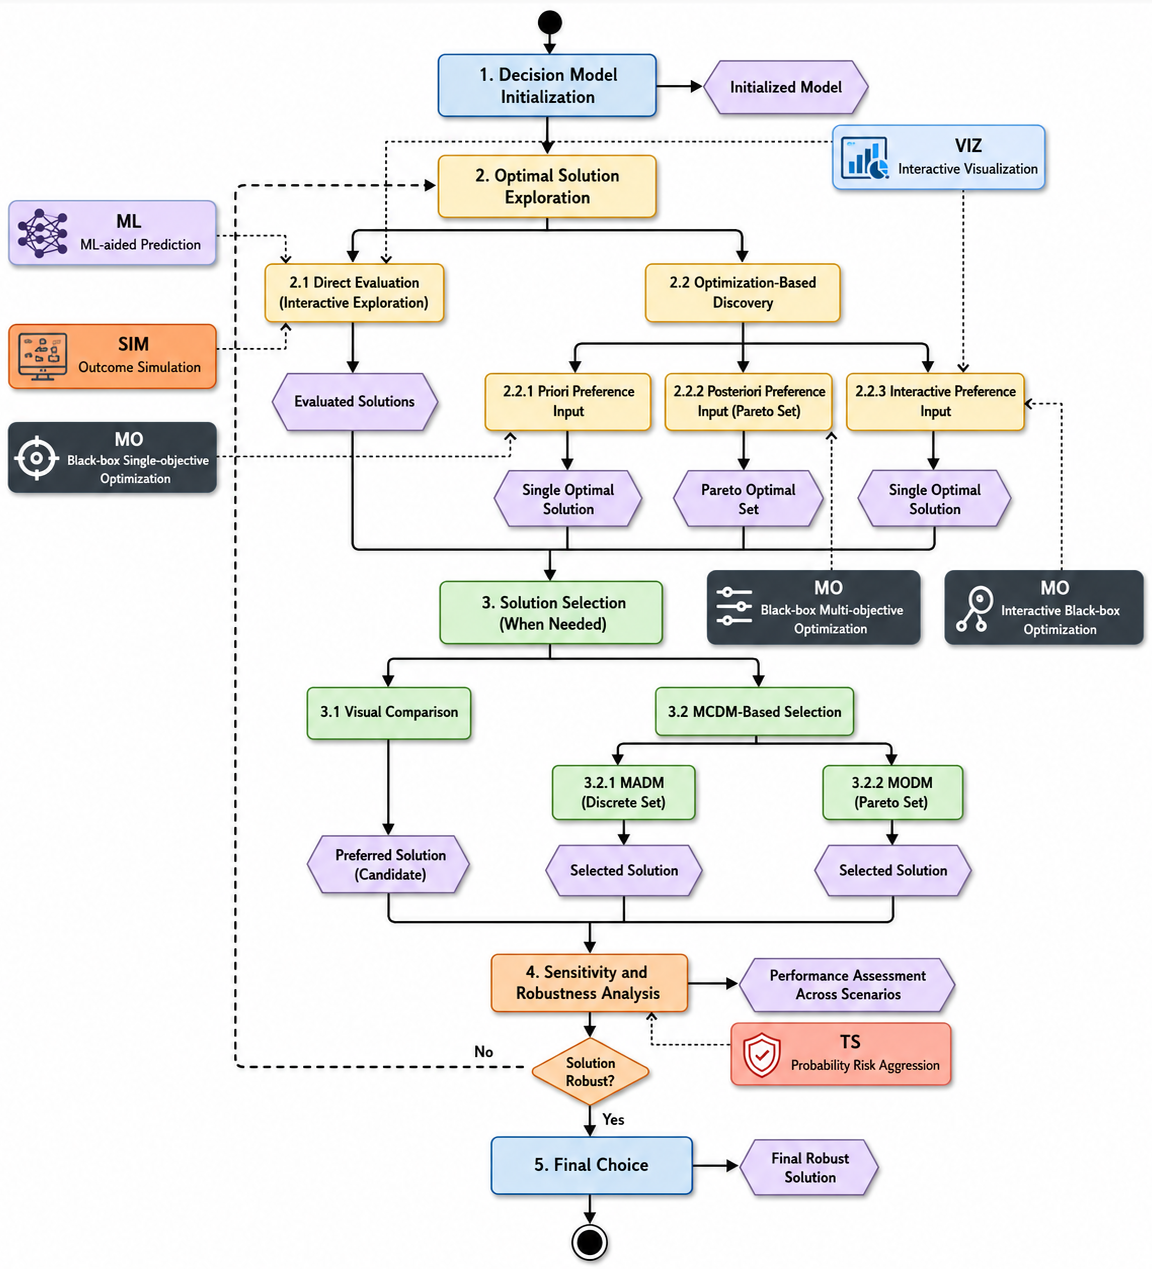
\includegraphics[width=0.98\textwidth]{Figures/ChoiceWorkflow.png}
\end{frame}

\begin{frame}{ICADOS Architecture}
  \begin{columns}[T,onlytextwidth]
    \column{0.42\textwidth}
    \begin{itemize}
      \item Causal and task specification.
      \item Evidence and model generation.
      \item Interactive decision support.
      \item Outcome simulation and comparison.
    \end{itemize}
    \column{0.58\textwidth}
    \centering
    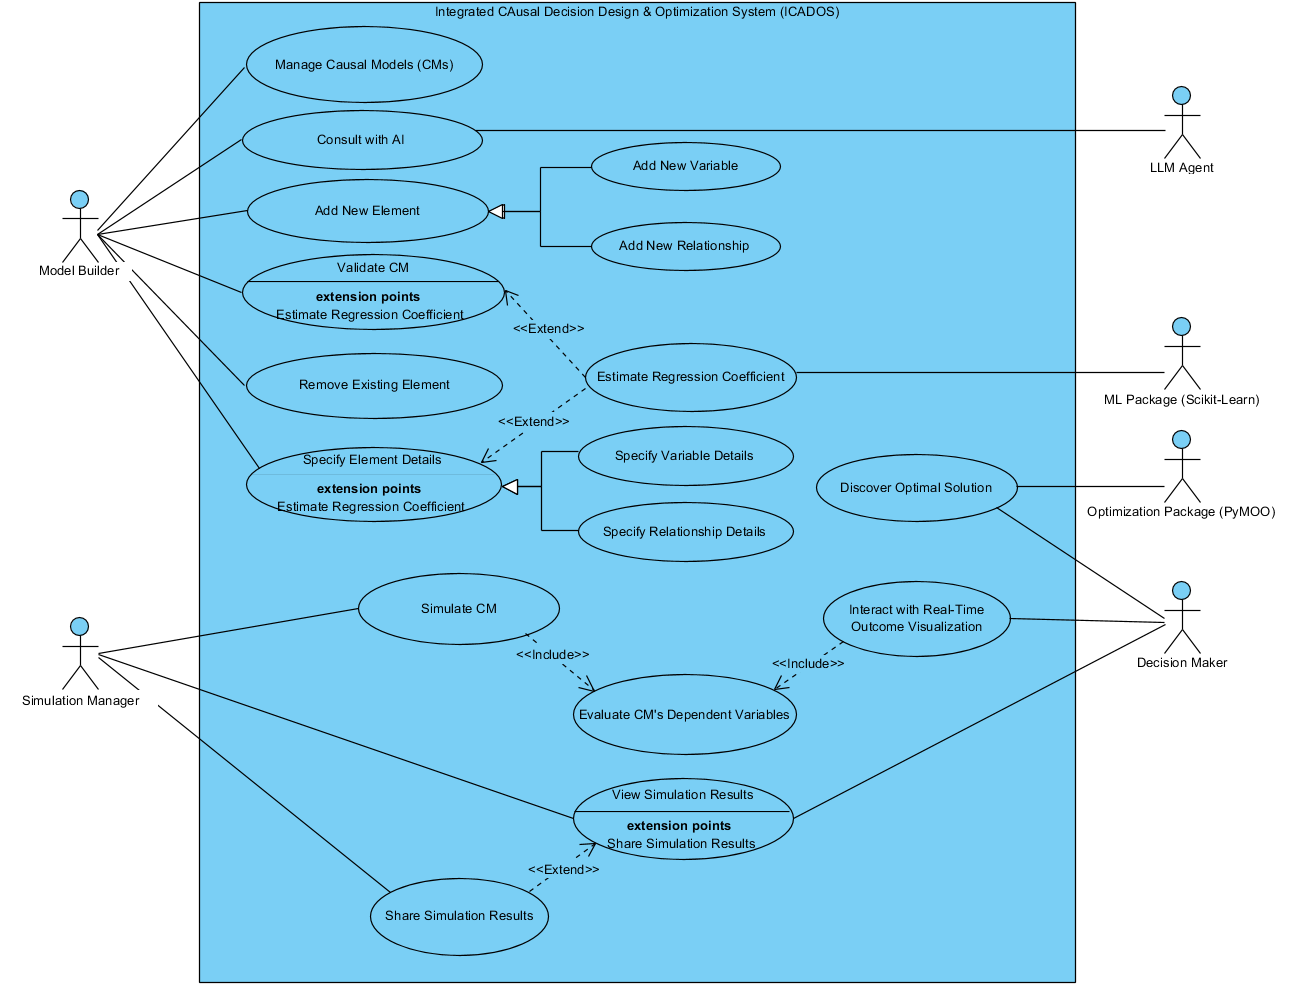
\includegraphics[width=0.95\textwidth]{Figures/ICADOS_UCD.png}
  \end{columns}
\end{frame}

\begin{frame}{Key Takeaways}
  \begin{columns}[T,onlytextwidth]
    \column{0.52\textwidth}
    \begin{itemize}
      \item Use tools for the decision task, not as a generic solution.
      \item Keep causal structure visible and testable.
      \item Support user reasoning rather than replace it.
      \item Combine prediction, optimization, simulation, and visualization.
      \item Evaluate recommendations for robustness, trust, and usability.
    \end{itemize}
    \column{0.48\textwidth}
    \centering
    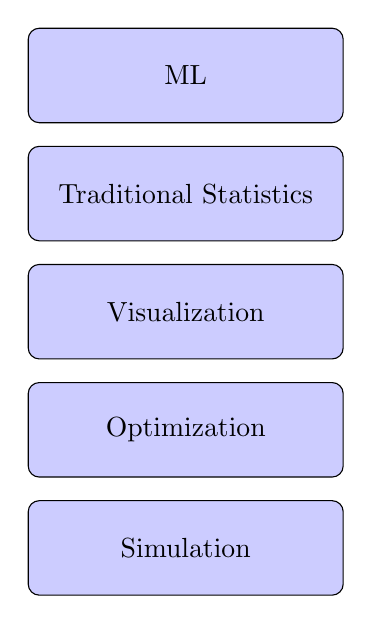
\begin{tikzpicture}
      \node[draw,fill=blue!20,rounded corners,minimum width=4cm,minimum height=1.2cm] {ML};
      \node[draw,fill=blue!20,rounded corners,minimum width=4cm,minimum height=1.2cm] at (0,-1.5) {Traditional Statistics};
      \node[draw,fill=blue!20,rounded corners,minimum width=4cm,minimum height=1.2cm] at (0,-3) {Visualization};
      \node[draw,fill=blue!20,rounded corners,minimum width=4cm,minimum height=1.2cm] at (0,-4.5) {Optimization};
      \node[draw,fill=blue!20,rounded corners,minimum width=4cm,minimum height=1.2cm] at (0,-6) {Simulation};
    \end{tikzpicture}
  \end{columns}
  \begin{center}
    \small Thank you.
  \end{center}
\end{frame}

\end{document}
